\documentclass[a4]{beamer}
\usepackage{amssymb}
\usepackage{graphicx}
\usepackage{subfigure}
\usepackage{newlfont}
\usepackage{amsmath,amsthm,amsfonts}
%\usepackage{beamerthemesplit}
\usepackage{pgf,pgfarrows,pgfnodes,pgfautomata,pgfheaps,pgfshade}
\usepackage{mathptmx}  % Font Family
\usepackage{helvet}   % Font Family
\usepackage{color}

\mode<presentation> {
 \usetheme{Default} % was
 \useinnertheme{rounded}
 \useoutertheme{infolines}
 \usefonttheme{serif}
 %\usecolortheme{wolverine}
% \usecolortheme{rose}
\usefonttheme{structurebold}
}

\setbeamercovered{dynamic}

\title[MA4704]{Technological Mathematics 4 \\ {\normalsize MA4704 Lecture 12A}}
\author[Kevin O'Brien]{Kevin O'Brien \\ {\scriptsize Kevin.obrien@ul.ie}}
\date{Spring Semester 2013}
\institute[Maths \& Stats]{Dept. of Mathematics \& Statistics, \\ University \textit{of} Limerick}

\renewcommand{\arraystretch}{1.5}

\begin{document}
\begin{frame}
\titlepage
\end{frame}
%----------------------------------------------------%
\begin{frame}
\frametitle{Example 1 (a)}
A rocket motor is manufactured by bonding together two types of
propellants, an igniter and a sustainer.
The shear strength of the bond (STRENGTH = y)
is thought to be related to the mean age of the propellants (MEAN AGE = x) when the motor is cast.
Fifteen observations were made giving the following scatter plot (next Slide).
\end{frame}

%----------------------------------------------------%
\begin{frame}
\frametitle{Example 1 (b)}

% image
% 12plot1
\begin{figure}
  % Requires \usepackage{graphicx}
  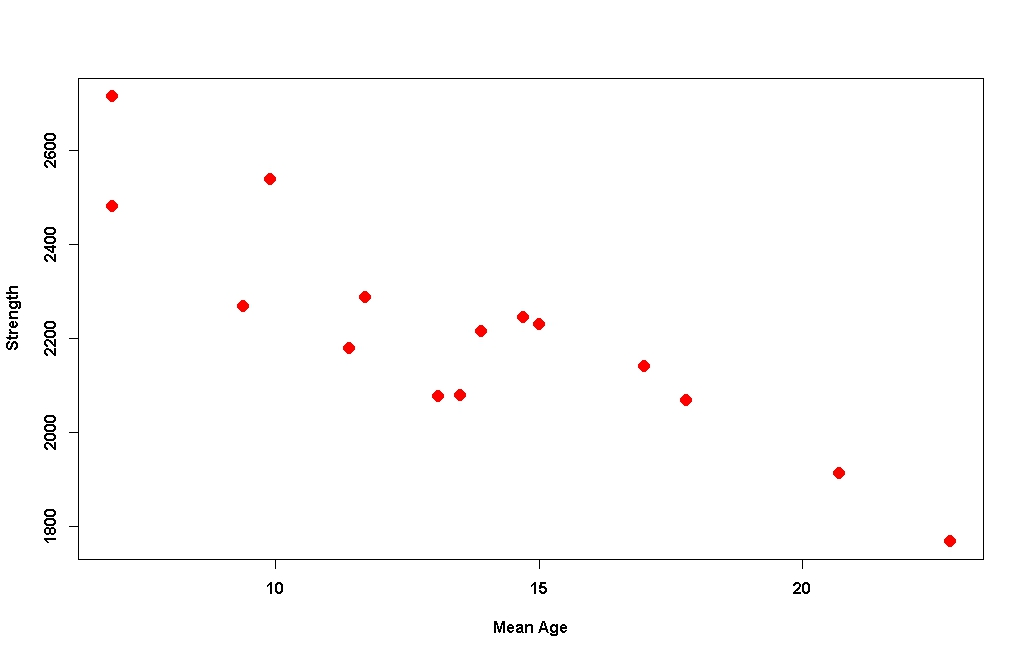
\includegraphics[scale=0.3]{12Aplot1}\\
\end{figure}

\end{frame}
%----------------------------------------------------%
\begin{frame}
\frametitle{Example 1 (c)}
\begin{itemize}
\item What sort of relationship is indicated by this scatterplot?
\item Strong or Weak?  - Quite Strong
\item Positive or Negative?  - Negative
\item Linear or Non-Linear - Seems to be linear
\end{itemize}
\end{frame}
%----------------------------------------------------%
\begin{frame}
\frametitle{Example 1 (d)}
Suppose we are given the following summations
\begin{itemize}
\item $\sum X = 213.4$
\item $\sum X^2 =3277.82$
\item $\sum Y = 34122$
\item $\sum Y^2 = 78547854$
\item $\sum XY = 472203.9$
\end{itemize}
Compute the mean values of $X$ and $Y$.

\[ \bar{x} = \frac{\sum x}{n} = \frac{213.4}{15} = 14.226 \]

Similarly $\bar{y} =  2274.8$

\end{frame}
%----------------------------------------------------%
\begin{frame}
\frametitle{Example 1 (e)}
Compute the \textbf{Sum of Squares Identities} ($S_{XX}$ , $S_{YY}$ and $S_{XY}$).\\

\bigskip
From Formula Sheet (Back of Exam Paper)
\begin{eqnarray*}
S_{XY} &=&
\sum x_iy_i - \frac{\sum x_i\sum y_i}{n} = \left[472203.9 - \frac{213.4 \times 34122}{15} \right]=  -13238.42\\
S_{XX} &=&
\sum x_i^2 - \frac{(\sum x_i)^2}{n} = \left[3277.82 - \frac{213.4^2}{15}\right] =  241.8493\\
S_{YY} &=&
\sum y_i^2 - \frac{(\sum y_i)^2}{n} = \left[78547854 - \frac{34122^2}{15}\right] = 927128.4\\
\end{eqnarray*}

\end{frame}

%----------------------------------------------------%
\begin{frame}
\frametitle{Example 1 (f)}
Compute the \textbf{Correlation Coefficient} $r_{XY}$

\[r_{XY} =  \frac{S_{XY}}{\sqrt{S_{XX} \times S_{YY}}} \]

\[r_{XY} =  \frac{-13238.42}{\sqrt{241.8493 \times 927128.4}} \]
Remark : $\sqrt{XY} = \sqrt{X} \times \sqrt{Y}$.
\[r_{XY} =  \frac{-13238.42}{\sqrt{241.8493} \times \sqrt{927128.4}} \]
\[r_{XY} =  \frac{-13238.42}{15.55 \times 962.87} = \frac{-13238.42}{14972.63} = -0.8841 \]

This value is consistent with our interpretation of the scatterplot: Strong Negative Linear Relationship.
\end{frame}
%----------------------------------------------------%

\begin{frame}
\frametitle{Example 1 (g)}
Calculate the least squares regression line.\\
\bigskip
The least squares regression line comprises two important estimates:
\begin{itemize}
\item  The slope estimate $b_1$
\item  The intercept estimate $b_0$.
\end{itemize}
The least squares regression line has the following form:

\[ \hat{y}  = b_0 + b_1x \]

$\hat{y}$ is the \textbf{predicted} value for variables Y, when given a particular value $x$ for the predictor variable X.
\end{frame}
%----------------------------------------------------%


\begin{frame}
\frametitle{Example 1 (h)}

\begin{itemize}
\item  The slope estimate $b_1$

\begin{eqnarray*}
b_1 = \frac{S_{XY}}{S_{XX}} = \frac{-13238.42}{241.8493} = -54.738
\end{eqnarray*}

\item  The intercept estimate $b_0$.
\begin{eqnarray*}
 b_0 = \bar{y} -b_1\bar{x} = 2274.8 - (-54.738 \times 14.226) = 3053.503
\end{eqnarray*}
\end{itemize}

\[ \hat{y}  = 3053.503 -54.738 x \]

\end{frame}
%----------------------------------------------------%
\begin{frame}
\frametitle{Example 1 (i)}
Interpret the values of the slope and the intercept.
\begin{itemize}
\item  The slope estimate $b_1$ :  For each additional year in age, the shear strength of the bond decreases by approximately 54 units.
\item The Intercept estimate $b_0$ : When the age of the propellant is 0 (i.e. brand new) the strength of the bond is expected to be 3053 units.
\end{itemize}
\bigskip
What is the estimate of the mean shear strength of the bond if the mean age of the propellants is 17 weeks?

\[ \hat{y}_{(x=17)}  = 3053.503 -54.738 \times 17 = 2122.96 \]

That looks plausible, from looking back at the scatter-plot.
\end{frame}

%----------------------------------------------------%
\begin{frame}
\frametitle{Example 1 (j)}

% image
% 12plot1
\begin{figure}
  % Requires \usepackage{graphicx}
  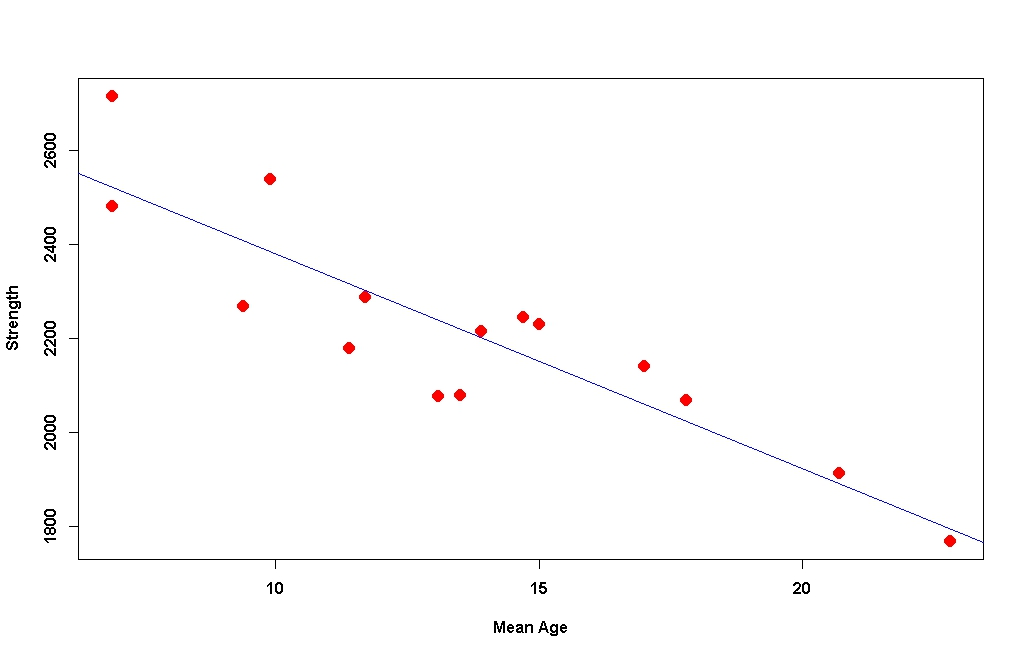
\includegraphics[scale=0.3]{12Aplot2}\\
\end{figure}

\end{frame}
%----------------------------------------------------%
\begin{frame}
\frametitle{Example 2 (a)}
(Spring 2010 Q5)\newline
A wood scientist wishes to determine if there is a relationship between the number of knots in a piece of wood and its tensile strength. A random selection of 8 timber beams were analysed and the results are given in the table (next slide).
\end{frame}
%----------------------------------------------------%
\begin{frame}
\frametitle{Example 2 (b)}
\begin{center}
\begin{tabular}{|c|c|c|}
\hline
% after \\: \hline or \cline{col1-col2} \cline{col3-col4} ...
Observation 	&	Number of knots (x) 	&	Tensile Strength 	\\
&		&	N.MS (y)	\\ \hline
A 	&	5	&	5	\\
B 	&	8	&	2.9	\\
C 	&	4	&	4.9	\\
D 	&	9	&	2.8	\\
E 	&	3	&	6.1	\\
F 	&	6	&	4.1	\\
G 	&	4	&	4.8	\\
H 	&	7	&	3.2	\\
  \hline
\end{tabular}
\end{center}

\end{frame}
%----------------------------------------------------%
\begin{frame}
\frametitle{Example 2 (c)}
Computing summations: recommended approach is construction of a table.\\
\begin{center}
\begin{tabular}{|c|c|c|c|c|c|}
  \hline
Obs	&	$X$	&	$Y$	&$X^2$	&$Y^2$	&	$XY$	\\
A 	&	5	&	5	&		&		&	25	      \\
B 	&	8	&	2.9	&		&		&	23.2	\\
C 	&	4	&	4.9	&		&		&	19.6	\\
D 	&	9	&	2.8	&		&		&	25.2	\\
E 	&	3	&	6.1	&		&		&	18.3	\\
F 	&	6	&	4.1	&		&		&	24.6	\\
G 	&	4	&	4.8	&		&		&	19.2	\\
H 	&	7	&	3.2	&		&		&	22.4	\\
(sum)&	46	&	33.8&		&		&	177.5	\\

  \hline
\end{tabular}
\end{center}

\end{frame}
%----------------------------------------------------%
\begin{frame}
\frametitle{Example 2 (d)}

Summations from previous slide.
\begin{itemize}
\item $\sum X = 46$
\item $\sum X^2 =296$
\item $\sum Y = 33.8$
\item $\sum Y^2 = 152.56$
\item $\sum XY = 117.5$
\end{itemize}
Compute the mean values of $X$ and $Y$.

\[ \bar{x} = \frac{\sum x}{n} = \frac{46}{8} = 5.75 \]

Similarly $\bar{y} =   4.225$
\end{frame}

%----------------------------------------------------%
\begin{frame}
\frametitle{Example 2 (f)}
Compute the \textbf{Sum of Squares Identities} ($S_{XX}$ , $S_{YY}$ and $S_{XY}$).\\
\bigskip
From Formula Sheet (Back of Exam Paper)
\begin{eqnarray*}
S_{XY} &=&
\sum x_iy_i - \frac{\sum x_i\sum y_i}{n} = -16.85\\
S_{XX} &=&
\sum x_i^2 - \frac{(\sum x_i)^2}{n} = 31.5\\
S_{YY} &=&
\sum y_i^2 - \frac{(\sum y_i)^2}{n} = 9.755\\
\end{eqnarray*}
\end{frame}
%----------------------------------------------------%

\begin{frame}
\frametitle{Example 2 (g)}
Compute the \textbf{Sum of Squares Identities} ($S_{XX}$ , $S_{YY}$ and $S_{XY}$).\\
\bigskip
From Formula Sheet (Back of Exam Paper)
\begin{eqnarray*}
S_{XY} &=&
\sum x_iy_i - \frac{\sum x_i\sum y_i}{n} = -16.85\\
S_{XX} &=&
\sum x_i^2 - \frac{(\sum x_i)^2}{n} = 31.5\\
S_{YY} &=&
\sum y_i^2 - \frac{(\sum y_i)^2}{n} = 9.755\\
\end{eqnarray*}
\end{frame}

\begin{frame}
\frametitle{Example 2 (h)}
Compute the regression estimates:
\begin{itemize}
\item  The slope estimate $b_1$

\begin{eqnarray*}
b_1 = \frac{S_{XY}}{S_{XX}} = \frac{-16.85}{31.5} = -0.5349
\end{eqnarray*}

\item  The intercept estimate $b_0$.
\begin{eqnarray*}
 b_0 = \bar{y} -b_1\bar{x} = 4.225 - (-0.5349 \times 5.75) = 7.300
\end{eqnarray*}
\end{itemize}

\[ \hat{y}  = 7.300 -0.5349 x \]

\end{frame}

%----------------------------------------------------%
\begin{frame}
\frametitle{Example 2 (i)}

% image
% 12plot1
\begin{figure}
  % Requires \usepackage{graphicx}
  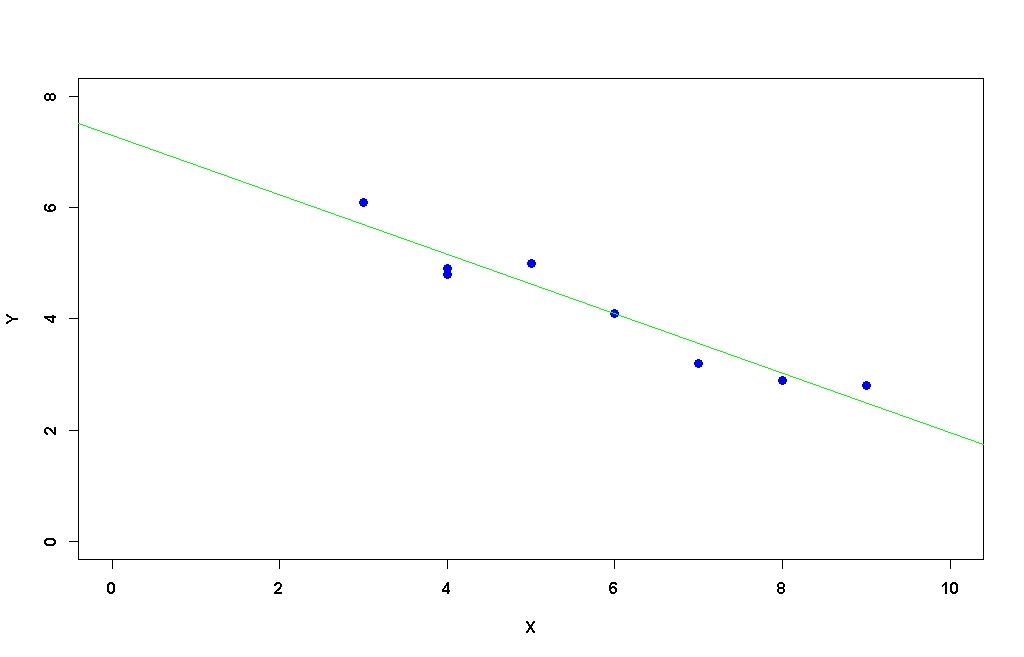
\includegraphics[scale=0.3]{12Aplot3}\\
\end{figure}

\end{frame}
\end{document}
%-----------------------------------------------------------------%

X=rnorm(15,12.08,sd=4)

Y=rnorm(15,2200,sd=200)

while(cor(X,Y)>(-0.875))
{
Y=rnorm(15,2200,sd=200)
}

X=round(X,1)
Y=floor(Y)


plot(X,Y,pch=17,col="blue",font.lab=2,font.axis=2,cex=1.6)
#
cor(X,Y)
sum(X)
sum(X^2)
sum(Y)
sum(Y^2)
sum(X*Y)


var(X)*(length(X)-1)
var(Y)*(length(Y)-1)
cov(X,Y)*(length(X)-1)
cor(X,Y)
coef(Y~X)
%-----------------------------------------------------------------% 